\documentclass[11pt, spanish, a4paper, twoside]{article}

% Versión 1.er cuat 2021 Víctor Bettachini < vbettachini@unlam.edu.ar >

\usepackage[T1]{fontenc}
\usepackage[utf8]{inputenc}

\usepackage[spanish, es-tabla]{babel}
% \def\spanishoptions{argentina} % Was macht dass?
% \usepackage{babelbib}
% \selectbiblanguage{spanish}
% \addto\shorthandsspanish{\spanishdeactivate{~<>}}


\usepackage{graphicx}
\graphicspath{{./figuras/}{../LaTeX/}{../figurasLaTeX/}}
% \usepackage{float}

\usepackage[arrowdel]{physics}
\newcommand{\pvec}[1]{\vec{#1}\mkern2mu\vphantom{#1}}
% \usepackage{units}
\usepackage[separate-uncertainty= true, multi-part-units= single, range-units= single, range-phrase= {~a~}, locale= FR]{siunitx}
\usepackage{isotope} % $\isotope[A][Z]{X}\to\isotope[A-4][Z-2]{Y}+\isotope[4][2]{\alpha}

\usepackage{tasks}
\usepackage[inline]{enumitem}
% \usepackage{enumerate}

\usepackage{hyperref}

% \usepackage{amsmath}
% \usepackage{amstext}
% \usepackage{amssymb}

\usepackage{tikz}
\usepackage{tikz-3dplot}
\usepackage{tikz-dimline}
\usetikzlibrary{calc}
% \usetikzlibrary{math}
\usetikzlibrary{arrows.meta}
\usetikzlibrary{snakes}
\usetikzlibrary{decorations}
\usetikzlibrary{decorations.pathmorphing}
\usetikzlibrary{patterns}

\usepackage[hmargin=1cm,vmargin=3cm, top= 0.75cm,nohead]{geometry}

\usepackage{lastpage}
\usepackage{fancyhdr}
\pagestyle{fancyplain}
\fancyhf{}
\setlength\headheight{28.7pt} 
\fancyhead[LE, LO]{\textbf{Mecánica Analítica Computacional} }
% \fancyhead[LE, LO]{\textbf{Mecánica General} }
\fancyhead[RE, RO]{\href{https://ingenieria.unlam.edu.ar/}{$\vcenter{\hbox{
\includegraphics[height=1cm]{ambos.pdf}}}$}}
\fancyfoot{\href{https://creativecommons.org/licenses/by-nc-sa/4.0/deed.es_ES}{$\vcenter{\hbox{
\includegraphics[height=0.4cm]{by-nc-sa_80x15.pdf}}}$} \href{https://ingenieria.unlam.edu.ar/}{DIIT - UNLaM}}
\fancyfoot[C]{ {\tiny Actualizado al \today} }
\fancyfoot[RO, LE]{Pág. \thepage/\pageref{LastPage}}
\renewcommand{\headrulewidth}{0pt}
\renewcommand{\footrulewidth}{0pt}



\begin{document}
\begin{center}
  % \textsc{\large Mecánica general}\\
  \textsc{\large Ligaduras}
\end{center}

\noindent
%De poder resolver estos problemas en forma autónoma puede asumir que adquirió los conocimientos mínimos sobre los temas abordados en la semana.
%No dude en consultar a docentes y compañeros si no puede terminarlos.
Los problemas marcados con (*) tienen alguna dificultad adicional, no dude en consultar.
\begin{enumerate}


\item 
\begin{minipage}[t][3.5cm]{0.68\textwidth}
	\textbf{Máquina de Atwood simple}\\
	Obtenga a partir de la ecuación de Euler-Lagrange la aceleración que presentan las pesas de masas \(m_1\) y \(m_2\) que cuelgan de una cuerda de longitud \(\ell\) que pasa por sobre una polea de radio \(R_p\) y masa \(m_p\).
	\begin{enumerate}
		\item Resuelva el caso en que se considera \(m_p\) irrelevante.
		\item Resuelva ahora considerando \(m_p\), y que la polea presenta una sección cilíndrica.
			El momento de inercia de tal cilindro de masa \(m\) ante rotaciones en torno a su eje de simetría longitudinal es \((m/2) R^2\).
	\end{enumerate}
\end{minipage}
\begin{minipage}[c][0.5cm][t]{0.3\textwidth}
	% \hspace{0.5cm}
	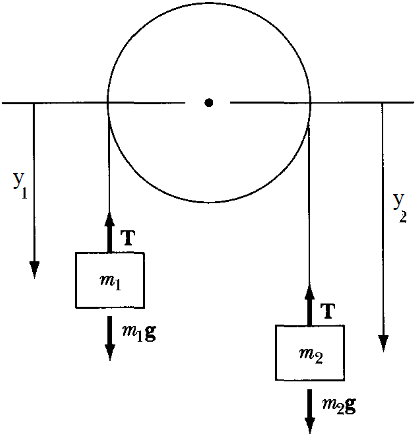
\includegraphics[width=0.75\textwidth]{marion_fig2_11a}
	% 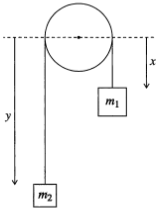
\includegraphics[width=0.75\textwidth]{marion_fig2_1a}
\end{minipage}


\item 
	\begin{minipage}[t][2.6cm]{0.8\textwidth}
		\textbf{Aro y polea}\\
		Una partícula de masa \(m\) pende de una sección de cuerda de longitud \(y_m\) que sobresale de una polea de radio \(R_p\) y masa despreciable.
		La cuerda tiene un longitud total \(\ell\), su  masa es despreciable y gira solidaria con la una polea.
		El otro extremo se ata con un nudo de masa \(M\) a un aro de masa \(m_a\), enrollándose parcialmente en torno a éste.
		El centro de la polea está a una altura \(h\) por sobre el del aro de radio \(R\) que como puede rotar libremente presenta un momento de inercia \(m_a R^2\).
		Denomine el ángulo desde el centro hasta el nudo medido desde la horizontal con \(\theta\). 
	\end{minipage}
	\begin{minipage}[c][0cm][t]{0.2\textwidth}
		% \hspace{0.5cm}
		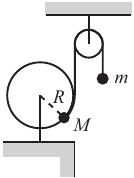
\includegraphics[width=0.75\textwidth]{cmchap6_fig6_14}
	\end{minipage}
	\begin{enumerate}
		\item Escriba la posición de las partículas con masa con origen el centro del aro.
		\item Describa la función de ligadura y utilícela para expresar las posiciones en función de \(\theta\).
		\item Obtenga la ecuación de Euler-Lagrange para la dinámica.\\
		Resultado:
		$R \left(- M R \ddot{\theta} + M g \cos{\left(\theta \right)} - R m \ddot{\theta} - R m_{a} \ddot{\theta} + g m\right) = 0$
	\end{enumerate}


\item 
\begin{minipage}[t][1.5cm]{0.7\textwidth}
	\textbf{Péndulo de pesas engarzadas y acopladas}\\ 
	Dos pesas de masa \(m_1\) y \(m_2\) están unidas por una barra rígida inextensible de longitud \(\ell\) y masa despreciable frente a las anteriores.
	La de \(m_1\) está engarzada en un eje horizontal y la de \(m_2\) en uno vertical.
\end{minipage}
\begin{minipage}[c][2cm][t]{0.3\textwidth}
	% \hspace{0.5cm}
	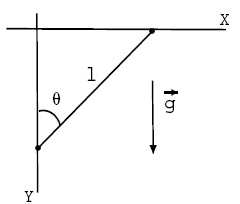
\includegraphics[width=0.75\textwidth]{fcen1-004}
\end{minipage}
\begin{enumerate}
	\item Escriba las posiciones de ambas partículas en función de una única coordenada haciendo uso de la ligadura que impone la barra rígida.
	Hágalo para:
	\begin{enumerate*}[
				%itemjoin=\quad,
				%before=\hspace*{\fill},
				%after=\hspace*{\labelwidth}\hspace*{-\labelsep}\hspace*{\fill},
			]
		\item \(y\), la coordenada para la pesa de \(m_2\),
		\item \(\theta\)
	\end{enumerate*} % https://tex.stackexchange.com/questions/591120/how-can-you-put-items-on-one-line-and-center-them
	\item Obtenga las aceleraciones y responda: ¿cuál coordenada generalizada preferiría?\\
	Resultado:
		$\ddot{y} = \frac{- \ell^{2} m_{1} y \dot{y}^{2} + g m_{2} \left(\ell^{2} - y^{2}\right)^{2}}{\ell^{4} m_{2} + \ell^{2} m_{1} y^{2} - 2 \ell^{2} m_{2} y^{2} - m_{1} y^{4} + m_{2} y^{4}}$
		\qquad
		$\ddot{\theta} = \frac{\left(\ell m_{1} \cos{\left(\theta \right)} \dot{\theta}^{2} - \ell m_{2} \cos{\left(\theta \right)} \dot{\theta}^{2} - g m_{2}\right) \sin{\left(\theta \right)}}{\ell \left(m_{1} \cos^{2}{\left(\theta \right)} + m_{2} \sin^{2}{\left(\theta \right)}\right)}$
	\item (*) ¿Cuál es el período de movimiento de pequeñas oscilaciones para el caso \(m_1 = m_2 = m\)?
\end{enumerate}



\item
\begin{minipage}[t][10cm]{0.6\textwidth}
	\textbf{Maquina de Atwood compuesta} [Marion (english) ex. 7.8]\\ 
	\begin{enumerate}
		\item Escriba la posición de las tres pesas y de la polea inferior en función de 
		las cuatro coordenadas generalizadas indicadas en la figura: \(y_i\) con \(i = 1,2,3,p\). 
		\item Modele las ligaduras que proveen las cuerdas en dos funciones.
		\item Haciendo uso de estas últimas reemplace en las posiciones para expresarles en función de solo dos \(y_i\).
		\item Calcule energías potenciales y cinéticas contemplando los momentos de inercia de las poleas.
		Recuerde la relacíón entre el perímetro (circunferencia) de un círculo y su radio para escribir la velocidad angular en función del \(\dot{y}_i\) correspondiente.
		\item Obtenga las dos ecuaciones de Euler-Lagrange.\\
		Resultados:\\
		$- g m_{1} + g m_{2} + g m_{3} + g m_{p} + m_{1} \ddot{y}_{1} + m_{2} \ddot{y}_{1} - m_{2} \ddot{y}_{2} + m_{3} \ddot{y}_{1} + m_{3} \ddot{y}_{2} + \frac{3 m_{p} \ddot{y}_{1}}{2} = 0$\\
		$- g m_{2} + g m_{3} - m_{2} \ddot{y}_{1} + m_{2} \ddot{y}_{2} + m_{3} \ddot{y}_{1} + m_{3} \ddot{y}_{2} + \frac{m_{p} \ddot{y}_{2}}{2} = 0$
		\item Resuelva este sistema de ecuaciones para obtener las dos correspondientes aceleraciones generalizadas y con estas escribir las aceleraciones de los cuatro cuerpos en cuestión.\\
		Resultados:\\
		$\ddot{y}_{1} = \frac{4 g m_{1} m_{2} + 4 g m_{1} m_{3} + 2 g m_{1} m_{p} - 16 g m_{2} m_{3} - 6 g m_{2} m_{p} - 6 g m_{3} m_{p} - 2 g m_{p}^{2}}{4 m_{1} m_{2} + 4 m_{1} m_{3} + 2 m_{1} m_{p} + 16 m_{2} m_{3} + 8 m_{2} m_{p} + 8 m_{3} m_{p} + 3 m_{p}^{2}}$\\
		$\ddot{y}_{2} = \frac{8 g m_{1} m_{2} - 8 g m_{1} m_{3} + 2 g m_{2} m_{p} - 2 g m_{3} m_{p}}{4 m_{1} m_{2} + 4 m_{1} m_{3} + 2 m_{1} m_{p} + 16 m_{2} m_{3} + 8 m_{2} m_{p} + 8 m_{3} m_{p} + 3 m_{p}^{2}}$\\
		$\ddot{y}_{3} = - \frac{8 g m_{1} m_{2} - 8 g m_{1} m_{3} + 2 g m_{2} m_{p} - 2 g m_{3} m_{p}}{4 m_{1} m_{2} + 4 m_{1} m_{3} + 2 m_{1} m_{p} + 16 m_{2} m_{3} + 8 m_{2} m_{p} + 8 m_{3} m_{p} + 3 m_{p}^{2}}$\\
		$\ddot{y}_{p} = - \frac{4 g m_{1} m_{2} + 4 g m_{1} m_{3} + 2 g m_{1} m_{p} - 16 g m_{2} m_{3} - 6 g m_{2} m_{p} - 6 g m_{3} m_{p} - 2 g m_{p}^{2}}{4 m_{1} m_{2} + 4 m_{1} m_{3} + 2 m_{1} m_{p} + 16 m_{2} m_{3} + 8 m_{2} m_{p} + 8 m_{3} m_{p} + 3 m_{p}^{2}}$
	\end{enumerate}
\end{minipage}
\begin{minipage}[c][0cm][t]{0.3\textwidth}
%		\begin{tikzpicture}
%			\draw [ultra thick] (-2,4) -- (2,4);
%			\fill [pattern = north east lines] (-2,4) rectangle (2,4.2); % techo
%			\draw (0,4) -- (0,3); % linea vertical techo - polea superior
%			\draw (0,3) circle [radius=0.5]; % polea superior
%			\draw (-0.5,3) -- (-0.5,1.5); % linea vertical izquierda polea sup - inf
%			\draw (0.5,3) -- (0.5,2.25); % linea vertical izquierda polea sup - m3
%			\draw (0.25,1.75) rectangle (0.75,2.25) node [anchor= north west] {\(m_3\)} ; % m3
%			% \draw (0.25,1.75) node [above=1, right=9.6] {\(m_3\)} rectangle (0.75,2.25) node [above=1, right=9.6] {\(m_3\)} ; % m3
%			\draw (-0.5,1.5) circle [radius=0.5]; % polea inferior
%			\draw (-1,1.5) -- (-1,.25); % linea vertical izquierda polea inf - m1
%			\draw (-1.25,-.25) rectangle (-0.75,0.25) node [anchor= north west] {\(m_1\)} ; % m1
%			\draw (0,1.5) -- (0,1); % linea vertical izquierda polea inf - m2
%			\draw (-.25,.5) rectangle (.25,1) node [anchor= north west] {\(m_2\)} ; % m2
%		\end{tikzpicture}
	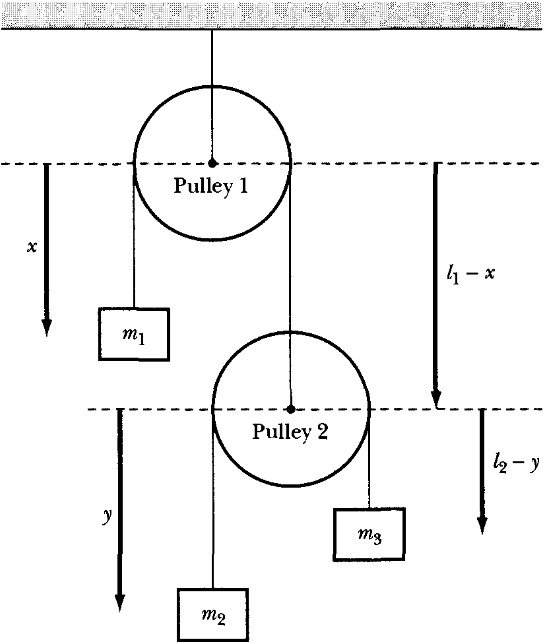
\includegraphics[width=\textwidth]{marion_fig7_6}
\end{minipage}



\end{enumerate}
\end{document}
